
\section{LSCVM: Immaculate Invasion}

	\subsection{Solution}

		\newcommand{\ttoc}[1]{\ttt{\bld{#1}}}

		The tool of choice for this challenge was \itl{Cutter}\footnote{\url{https://github.com/radareorg/cutter}}, an open-source
		reverse-engineering framework which performs disassembly, function analysis, and function/value renaming, among other things.

		\begin{figure}[!htbp]\centering
			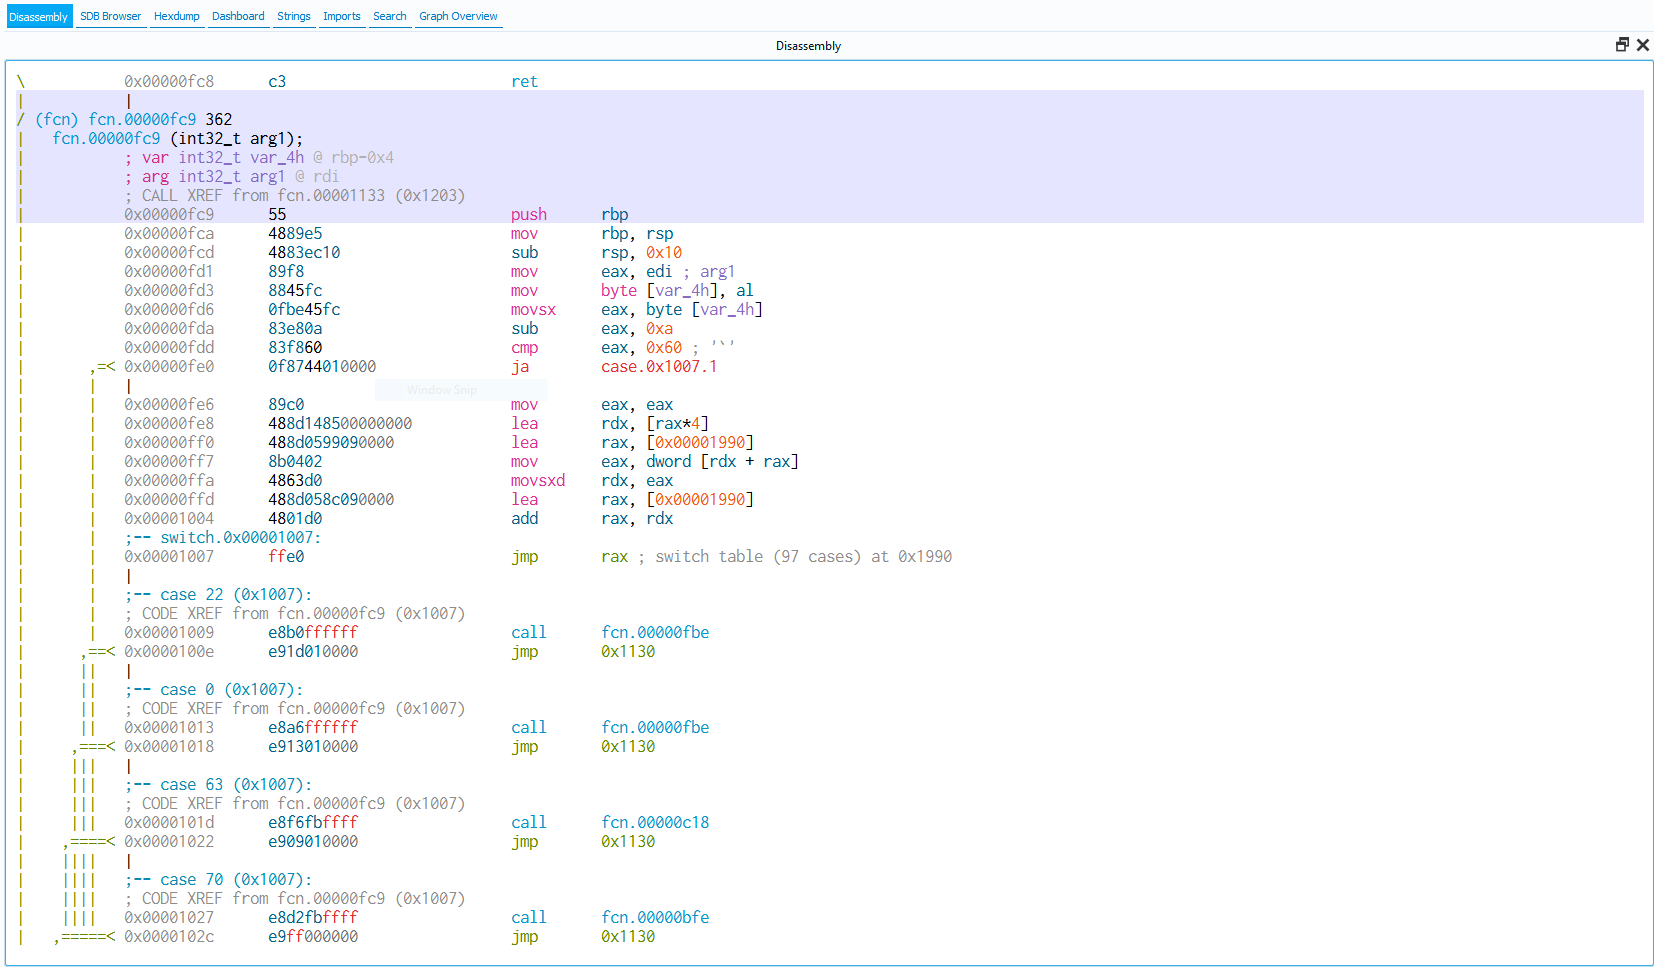
\includegraphics[width=150mm]{figures/lscvm-ii/cutter-screenshot.png} \vspace{5mm}
			\caption{A screenshot of Cutter}
			\label{fig:jumptable}
		\end{figure}

		The first hurdle was getting the program to run beyond its error message of \ttt{[-] Flag file open error}; upon
		inspection of the disassembly, the program tries to open a file named \enquote{flag}, which presumably contains the
		flag on the server-side --- \mintinline{sh}{$ touch flag} convinced the program to start.

		\pagebreak
		Given that the program asks for a login ID, the next step was to check for strings and \ttt{strcmp}s in the code,
		and one was indeed found:

		\begin{figure}[!htbp]\centering
			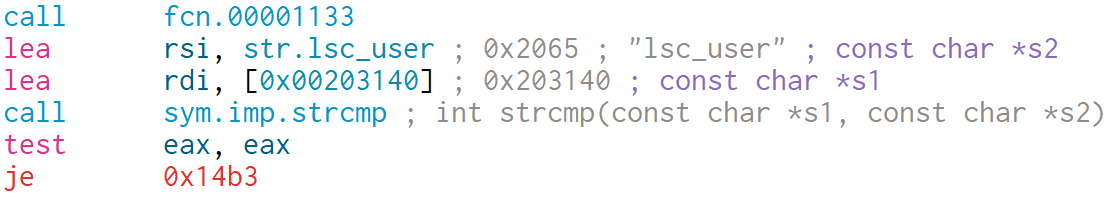
\includegraphics[width=150mm]{figures/lscvm-ii/user-strcmp.png} \vspace{5mm}
			\caption{A suspicious \ttt{strcmp}}
		\end{figure}

		Of course, no challenge is so easy, especially one that sat at above 950 points more than 24 hours after the qualifiers started. On
		further inspection, the operand of \ttt{strcmp} appeared to be the output of a call to \ttt{fcn.00001133}, which itself
		took some very long and suspicious strings as input: \ttt{eiMaAghMcAgjcMMdAgjcMMaAgjcMMaAhhcMMdAijMaAcfMPPPPPPPP}.

		Another discovery was this instruction: \mintinline{nasm}{cmp dword [var\_1174h], 2}, where \ttt{var\_1174h} contained the value
		of \ttt{argc}. Passing a second argument in the invocation (eg. \mintinline{sh}{$ ./lscvm-ii x}) revealed a \itl{very} useful
		debugging mode that printed what appeared to be a stack.

		Following the call chain eventually led to the jump table for opcode dispatch, pictured in Figure \ref{fig:jumptable}. Some quick
		analysis revealed that this was a indeed stack-based virtual machine (\itl{thankfully}). Combined with the debugging output, and the
		fact that the text output (the banner, login prompt, etc.) was printed using the VM instead of say \ttt{printf}, some basic opcodes
		were decoded:

		\begin{nicetable}[1.3][0.6\textwidth]{ X[c,m] | X[c,m] | X[c,m] | X[3,c,m] }
			Opcode              &   Pops            &   Pushes              &   Description \\ \hline
			\ttoc{u} to \ttoc{u}&   --              &   \ttt{0} to \ttt{9}  &   constant    \\
			\ttoc{A}            &   \ttt{a}, \ttt{b}&   \ttt{a + b}         &   add         \\
			\ttoc{M}            &   \ttt{a}, \ttt{b}&   \ttt{a * b}         &   multiply    \\
			\ttoc{P}            &   \ttt{a}         &   --                  &   \ttt{printf("\%c",a)} \\
		\end{nicetable}

		Piecing things together, it was inferred that we were most likely supposed to input a \itl{program} when asked for the user ID,
		which would then print \ttt{lsc\_user} as required. Given that ASCII values for the lowercase alphabets start at 97, a small
		program was quickly written that would take in a string and output opcodes that would print it (Listing \ref{code:lscvm-deasciiinator}).

		After trying it out, however, we were quickly met with disappointment, as we were faced with our old friend \ttt{[-] Wrong id}.

		\pagebreak
		After more digging, the user id was expected to be at the memory address \ttt{0x203140}; using the renaming feature of Cutter, we could
		make it easier to spot:

		\begin{figure}[!htbp]\centering
			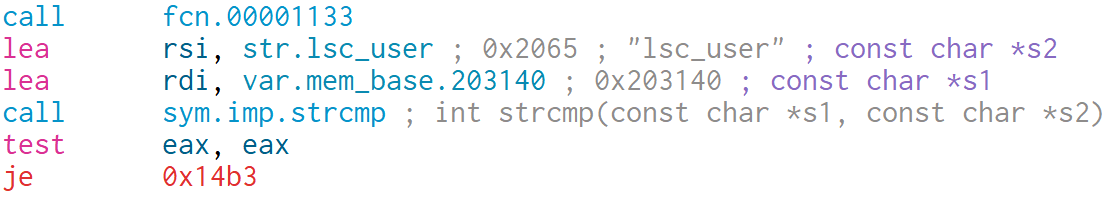
\includegraphics[width=150mm]{figures/lscvm-ii/addr-after-rename.png} \vspace{5mm}
			\caption{\ttt{[0x203140]} after being renamed into \ttt{var.mem\_base.203140}}
		\end{figure}

		Scrolling through the opcode list while looking for the address (now renamed) yielded this very interesting function, mapped to opcode
		\ttt{K}:

		\begin{figure}[!htbp]\centering
			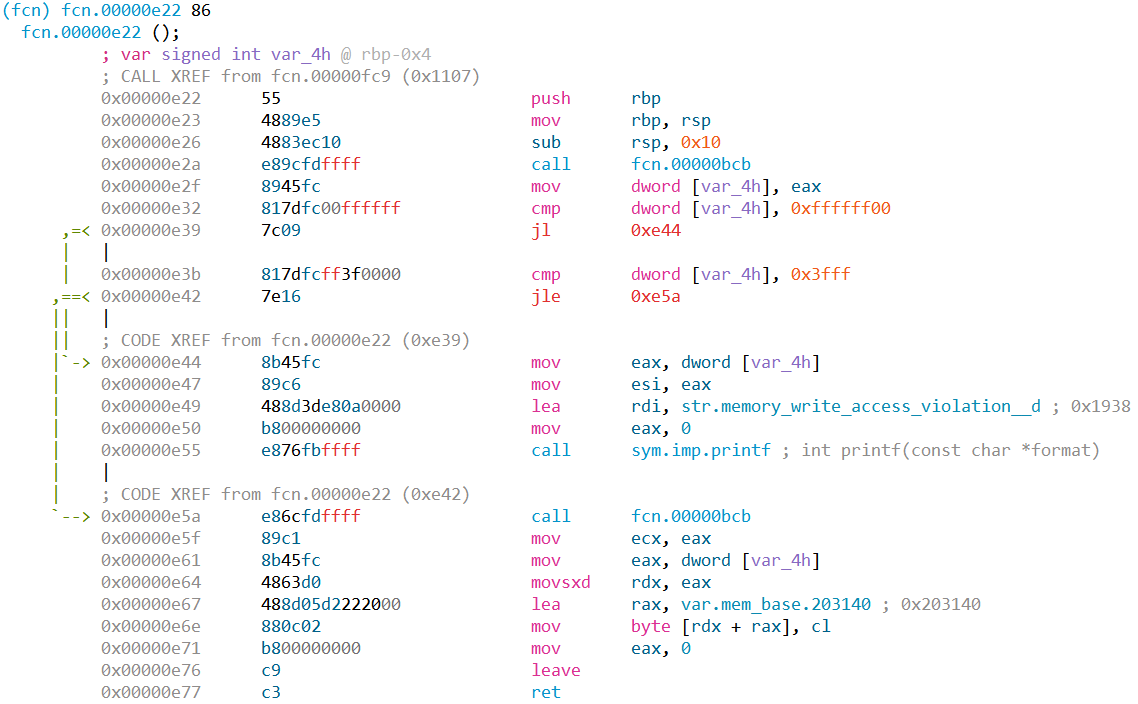
\includegraphics[width=150mm]{figures/lscvm-ii/write-to-memory.png} \vspace{5mm}
			\caption{A function to \sout{surpass metal gear} write to memory?}
		\end{figure}

		There was also an accompanying opcode \ttoc{E}, which read a value from memory. The memory buffer appeared to be an array of 32-bit
		values, and opcodes \ttoc{K} and \ttoc{E} took an index into this array. Slight modifications were made to \ttt{lscvm-deasciiinator}
		to yield \ttt{lscvm-memoryinator} (basically keeping track of an offset and replacing \enquote{P} with \enquote{K}), which would
		generate opcodes to write a string into a given offset in memory.

		\pagebreak
		Finally, then, the challenge could be solved (the password was also in plain sight, \ttt{hi\_darkspeed-corp!}):

		\begin{listing}[!htbp]
			\begin{minted}[autogobble,xleftmargin=0.075\textwidth,xrightmargin=0.075\textwidth,frame=leftline,framesep=4mm,framerule=0.4mm]{sh}
				$ ./lscvm-memoryinator
				string: lsc_user
				address: 0

				ggdMMaKfgAfMcMfAbKjjMjAjAcKgfdMMfAdKfgAfMcMhAeKfgAfMcMfAfKcf
				McfMMbAgKfgAfMcMeAhK

				string: hi_darkspeed-corp!
				address: 0

				jeAiMaKhdfMMbKgfdMMfAcKcfMcfMMdKjjMjAhAeKfgAfMcMeAfKhdfMMcAg
				KfgAfMcMfAhKfgAfMcMcAiKcfMcfMMbAjKcfMcfMMbAcfMKcfMcfMMbcfMMb
				AKfddMMbcfMMcAKjjMjAjAbcfMMdAKfgAfMcMbAbcfMMeAKfgAfMcMeAbcfM
				MfAKfgAfMcMcAbcfMMgAKfgAdMbcfMMhAK
				^C

				$ nc lscvm-ii.cddc19q.ctf.sg 9001

				=== Welcome to LSCVM(LightSpeed Corp Virtual Machine) ===
				ID : ggd...AhK
				Password : jeA...hAK

				Login Successful! $CDDC19${IcY_GrE37ings_Fr0M_LigHT5pEeDC0Rp}

				lsc_user, Good Bye!
			\end{minted}
		\end{listing}

	% end subsection


	\subsection{Flag}
		The flag for this challenge was \cddcflag{IcY\_GrE37ings\_Fr0M\_LigHT5pEeDC0Rp}.
	% end subsection


	\subsection{Further Analysis}
		While we were unable to actually come up with a quine to submit for the next LSCVM challenge (Quintessential Harlequin), we
		continued to take apart the VM (on the advice that it would be used again in the Finals!), since solving \ttt{lscvm-ii} did
		not require all of the opcodes (far from it).

		Again, the renaming feature of Cutter was extremely helpful, and we were able to discover the address of the program counter, the
		base address of the stack, and (in the case of \ttt{lscvm-qh}), the mirror of stdout. Each buffer appears to be a identical
		with a fixed size of \ttt{0x4e200} bytes (\ttt{0x13880} 32-bit words), and the number of items stored after the last
		element (ie. at offset \ttt{0x4e200} from the base address).

		We (eventually) managed to decipher all of the opcodes and their purpose:


		\begin{nicetable}[1.3][0.9\textwidth]{ X[.7,c,m] | X[c,m] | X[c,m] | @{\hspace{1.5em}}X[3,l,m] }
			Opcode              &   Pops                &   Pushes              &   \multicolumn{1}{c}{Description} \\ \hline
			\ttoc{a} to \ttoc{j}&   --                  &   \ttt{0} to \ttt{9}  &   constant                                    \\
			\ttoc{A}            &   \ttt{a}, \ttt{b}    &   \ttt{a + b}         &   add                                         \\
			\ttoc{B}            &   --                  &                       &   stop execution immediately                  \\
			\ttoc{C}            &   \ttt{x}             &   --                  &   call (jump to absolute instruction \ttt{x}) \\
			\ttoc{D}            &   \ttt{x}             &   --                  &   pop (drop)                                  \\
			\ttoc{E}            &   \ttt{addr}          &   \ttt{value}         &   read memory from \ttt{addr}                 \\
			\ttoc{F}            &   \ttt{ofs}           &   \ttt{value}         &   fetch from stack (\ttt{ofs} elms below top) \\
			\ttoc{G}            &   \ttt{ofs}           &   --                  &   relative jump forward                       \\
			\ttoc{H}            &   \ttt{ofs}           &   \ttt{value}         &   same as \ttoc{F}, but removes the element   \\
			\ttoc{I}            &   \ttt{x}             &   --                  &   \ttt{printf("\%d",x)}                       \\
			\ttoc{J}            &   \ttt{a}, \ttt{b}    &   \ttt{cmp}           &   $-1$ if $a<b$, $0$ if $a=b$, $1$ if $a>b$   \\
			\ttoc{K}            &   \ttt{val}, \ttt{addr}&  --                  &   writes \ttt{val} to memory at \ttt{addr}    \\
			\ttoc{M}            &   \ttt{a}, \ttt{b}    &   \ttt{a * b}         &   multiply                                    \\
			\ttoc{P}            &   \ttt{x}             &   --                  &   \ttt{printf("\%c",x)}                       \\
			\ttoc{R}            &   --                  &   --                  &   return                                      \\
			\ttoc{S}            &   \ttt{a}, \ttt{b}    &   \ttt{a - b}         &   subtract                                    \\
			\ttoc{V}            &   \ttt{a}, \ttt{b}    &   \ttt{a / b}         &   integer divide                              \\
			\ttoc{Z}            &   \ttt{cond}, \ttt{ofs}&  --                  &   jump (relative) if \ttt{cond} is $0$
		\end{nicetable}

		Of note are the \ttoc{C} and \ttoc{R} opcodes, which \itl{call} and \itl{return} respectively. There is another array which
		is only accessed by these instructions that functions as a \itl{callstack}. \ttoc{C} pushes the current program counter ($PC$)
		to this callstack, and \ttoc{R} pops the return address from the callstack, and sets $PC$ to it, moving execution back to the
		callsite.


		% \undef\ttoc


	% end subsection


% end section


















